\documentclass[a4paper,12pt]{article}
\usepackage[T1]{fontenc}
\usepackage{imakeidx}
\usepackage{graphicx}
%\makeindex[columns=3, title=Alphabetical Index, intoc]

\begin{document}

\textbf{Soft and Hard skills}


\tableofcontents
\clearpage

 
\section{Introduction}
This document lists a set of soft and hard skills I'm thinking it might be good to achieve during the apprenticeship at akhter computers. The when this document has been created was the 24th February 2022

\section{soft skills}
These are the skills to fit in at a workplace. Soft skills are so important that they are often the reason employers decide whether to keep or promote an employee.They include personality, attitude, flexibility, motivation, and manners.

Take him for example:

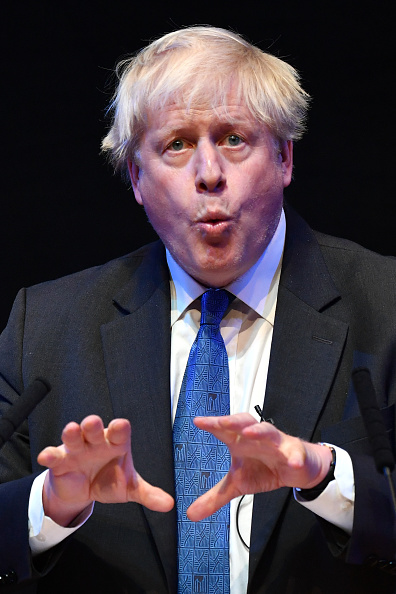
\includegraphics[width=3cm]{./boris-soft.jpg}

\includegraphics[width=6cm]{./boris-soft3.jpg}
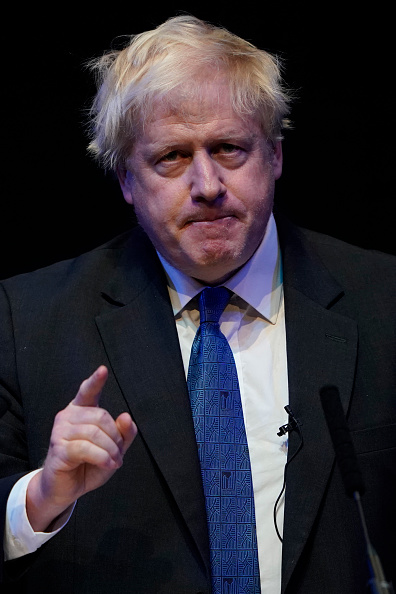
\includegraphics[width=3cm]{./boris-soft2.jpg}

He's got personality, attitude, flexibility, motivation and especially fantastic manners.

An other important soft skill for a prime minister might be \emph{not to dodge questions}.
One of the most common failures has been those attempts to avoid difficult questions, often by trying to answering something completely different.
Dodging the challenging questions is never a good approach, regardless of whether or not the spokesperson is involved in politics, and can result in questions being asked repeatedly by the reporter, which then becomes the focus of the interview.

\clearpage

\section{hard skills}
Hard skills (or technical skills), are directly relevant to the job. These are often more quantifiable, and easier to learn than soft skills.
A few examples of hard skills for a prime minister, might be the ability to understand:

\begin{itemize}

\item  how governments function 
\item  how decisions are made,
\item  how economic policies are formulated,
\item  how rules affect outcomes and broaden the horizons of graduates

\end{itemize}



\section{soft skills I want to achieve}

\subsection{communication}

\begin{itemize}
\item Being able to say crystal clear what are the PROs and CONs of a situation I'm facing without suffering in silence.
\item to be able to speak clearly and politely with people in person, by phone, and in writing.
\end{itemize}

\subsection{become a good listener}
\begin{itemize}
\item Fully understand what others want to communicate, particularly when the statement lacks clarity.
\item Listening demands the attempt to decode and interpret verbal messages and nonverbal cues, like tone of voice, facial expressions, and physical posture
\item Ask questions
\item Communicating I'm listening through body language
\item Allowing the speaker to complete each sentence before responding. Do not interrupt and genuinely answer the question.
\end{itemize}

\section{Hard skills I want to achieve}
Before getting a job for akhter computer I came across hundres of vacancies and many of them had things like JSON, Maven, Meteor, Kubernetes, Azure etc...

\subsection{JSON}
I wish to understand once for all what JSON is.
\begin {itemize}
\item Why it's needed
\item Where can it be used in my working environment
\item Why is it so popular
\end {itemize}

\subsection{C++}
Ideally learn C++ so I can refresh the technical side I've almost totally forgot and in the meantime starting to develop a third not-mentioned soft skill which is co-operation. Usually many problems arise when working on the same file on github. When this happens we have to sit and talk. So this is a technical skill but the reason I'm chosing it is to see how well I do in scenarios where communication is crucially needed
\clearpage

\printindex

\end{document}
